\chapter{Welded knots, isometry Lie algebras and arrow diagrams}
\label{ch:welded-knots-isometry-lie-algebras-and-arrow-diagrams}

\lettrine{\libertineInitialGlyph{T}}{aken} generally, knot theory is the study of codimension two embedded submanifolds. Welded knots, or \(w\)-knots are a diagrammatic generalisation of knots that relate to codimension two knotted objects in \(\mathbb{R}^{4}\), rather than \(\mathbb{R}^{3}\), and they have their own flavour of Vassiliev invariants and the corresponding theory.

Generalisations of the Vassiliev invariants to objects other than knotted circles in \(\mathbb{R}^{3}\) take the name \textbf{finite type invariants}. On one hand, welded knots are more complicated topological objects, relating to ribbon embeddings of tori in four dimensions. On the other hand however their finite type invariant theory is much more manageable than the classical case, so studying the simpler, welded version of \(\mathcal{A}\) may shed light on how to study the algebra \(\mathcal{A}\), as well as being interesting in its own right.

\section{Welded knots}

A good and thorough exposition of the theory of welded knots is \cite{finite-type-invariants-of-w-knotted-objects-I-w-knots-and-the-alexander-polynomial, finite-type-invariants-of-w-knotted-objects-II-tangles-foams-and-the-kashiwara-vergne-problem}. Their presentation is in terms of virtual knots and circuit algebras.

The definition of classical knots is first and foremost topological: they are ambient isotopy classes of embeddings of oriented circles into \(\mathbb{R}^{3}\). Due to the Reidemeister theorem, we may instead work with equivalence classes of planar knot diagrams under the Reidemeister moves.

With welded knots, the definition is the other way around. We will define them diagrammatically as equivalence classes of planar knot diagrams under an extended set of Reidemeister moves.

\begin{definition}
	A \textbf{welded knot} is an immersed curve in \(\mathbb{R}^{3}\), where each four-valent planar vertex is decorated by a vertex of one of the following types, respecting the orientation of the planar curve.
	\[\poscross\;, \quad \negcross\;, \quad \virtcross\]
	The third crossing type is called a \textbf{virtual crossing}.

	The equivalence relations are planar isotopy and:
	\begin{enumerate}
		\item The \textbf{(framed) Reidemeister moves}
			\begin{equation}
				\tag{\ronef, \rtwo, \rthree}
				\def\svgscale{0.34}
				\adjustbox{valign=c}{\input{graphics/reidemeister_1_framed.pdf_tex}}
				\; \;
				,
				\qquad
				\def\svgscale{0.34}
				\adjustbox{valign=c}{\input{graphics/reidemeister_2.pdf_tex}}
				\; \;
				,
				\qquad
				\def\svgscale{0.34}
				\adjustbox{valign=c}{\input{graphics/reidemeister_3.pdf_tex}}
			\end{equation}
		\item The \textbf{virtual Reidemeister moves}
			\begin{equation}
				\tag{\vrone, \vrtwo, \vrthree}
				\def\svgscale{0.34}
				\adjustbox{valign=c}{\input{graphics/reidemeister_virtual_1_framed.pdf_tex}}
				\; \;
				,
				\qquad
				\def\svgscale{0.34}
				\adjustbox{valign=c}{\input{graphics/reidemeister_virtual_2.pdf_tex}}
				\; \;
				,
				\qquad
				\def\svgscale{0.34}
				\adjustbox{valign=c}{\input{graphics/reidemeister_virtual_3.pdf_tex}}
				\; \;
				,
			\end{equation}
			\begin{equation}
				\tag{\vrfour}
				\def\svgscale{0.34}
				\adjustbox{valign=c}{\input{graphics/reidemeister_virtual_4.pdf_tex}}
			\end{equation}
		\item The \textbf{overcrossings commute} relation
			\begin{equation}
				\label{eq:OC}
				\tag{\oc}
				\def\svgscale{0.34}
				\adjustbox{valign=c}{\input{graphics/reidemeister_overcrossings_commute.pdf_tex}}
			\end{equation}
	\end{enumerate}
	\begin{remarks}
		\begin{enumerate}
			\item There should technically be two variants of \(\ronef\), another in which all crossings are changed, and the same is true for \(\vrfour\). This is even before orientation is taken into account: all of the moves are true for each choice of orientation of each strand.
			\item The moves \(\vrone\), \(\vrtwo\) and \(\vrthree\) govern how virtual crossings interact with each other. The move \(\vrfour\) governs how virtual crossings interact with classical crossings. It implies that strands consisting of only virtual crossings may be freely rerouted around classical crossings. The interpretation of this fact can be found in \cite{virtual-knot-theory}.
			\item In the \ref{eq:OC} relation, the order of the two overcrossings along the middle strand changes, hence the name. The version of \ref{eq:OC} in which the crossings are changed is called \textbf{undercrossings commute} and is \textit{not} an imposed relation: undercrossings do \textit{not} commute for welded knots. Indeed, allowing undercrossings to commute would trivialise welded knots. For an explanation of why this lack of symmetry is to be expected in terms of the tube map which we are about to define, the curious reader is referred to \cite[Sec. 2.2]{finite-type-invariants-of-w-knotted-objects-I-w-knots-and-the-alexander-polynomial}.
		\end{enumerate}
	\end{remarks}
\end{definition}

There is also a topological interpretation of welded knots, but it is not known exactly how well the topological object represents the diagrammatic one: welded knots are ambient isotopy classes of ribbon-embedded tori in \(\mathbb{R}^{4}\), up to some global orientation reversal move, and potentially some further moves \cite{virtual-knot-presentation-of-ribbon-torus-knots}. The map from welded knots to ribbon embedded tori is known as the tube map. We do not discuss the details here, instead referring the reader to \cite{on-the-welded-tube-map}. However this doesn't particularly matter: we define finite type invariants of welded knots from their diagrammatic definition, remaining confident that welded knots topologically correspond to something close to ribbon-knotted tori modulo a global orientation reversal move in \(\mathbb{R}^{4}\).

In fact, we can even avoid the trouble of the global orientation reversal move by passing to welded long knots.

\begin{definition}
	A (classical) \textbf{long knot} is the same as a knot, but instead of being an embedding of the circle \(S^{1} \hookrightarrow \mathbb{R}^{3}\), it's an embedding of the line \(k: \mathbb{R} \hookrightarrow \mathbb{R}^{3}\), with the condition that \(k(t) = (t, 0, 0)\) for all large \(|t|\).
\end{definition}

Similarly, we define welded long knots.

\begin{definition}
	A \textbf{welded long knot} is a welded knot, but instead of a planar curve it is a planar immersion \(\ell: \mathbb{R} \to \mathbb{R}^{2}\) such that \(\ell(t) = (t, 0)\) for all large \(|t|\).
\end{definition}

For why this stops the global orientation reversal we refer the reader again to \cite{virtual-knot-presentation-of-ribbon-torus-knots} and also \cite[Corrigendum]{finite-type-invariants-of-w-knotted-objects-II-tangles-foams-and-the-kashiwara-vergne-problem}.

For the finite type theory, the algebra \(\mathcal{A}\) of Jacobi diagrams (and chord diagrams), is replaced with \(\mathcal{A}(|)\). The relations are the exact same (either \ref{eq:IHX} or \ref{eq:4T}), but instead of the univalent vertices having a cyclic order (and and the skeleton being a circle) they have a linear order (and the skeleton is a line).

\section{Arrow diagrams}

The finite type theory of welded long knots is similar to that of classical long knots.

\begin{definition}
	A \textbf{singular welded long knot} is a welded long knot whose crossings can also be of the following types
	\[\semivirtposcross \;, \quad \semivirtnegcross.\]
	They are known as \textbf{positive semi-virtual crossings} and \textbf{negative semi-virtual crossings}, and they correspond to topological singularities of ribbon-knotted tori.

	% FIX: There's probably better notation.
	The set of \(m\)-singular welded long knots forms an algebra with the product given by connected sum given by concatenation and coproduct \(\Delta(k) = k \otimes k\). This is called the \textbf{algebra of \(m\)-singular welded long knots}, \(\mathcal{K}_{w, m}^{\bullet}(|)\).

	The algebra of \(0\)-singular welded long knots, or just the algebra of welded long knots \(\mathcal{K}^{\bullet}_{w, 0}(|) = \mathcal{K}_{w}(|)\) is filtered by the images of succesive powers of \(\partial\), and the filtration is compatible with the bialgebra structure.
\end{definition}

Just like in the classical case, the notions of invariants of \(m\)-singular welded long knots, their differentiability, and the derivative and boundary operators transfer over the the welded case. However now the derivative and boundary depend on the type of singularity.

\begin{align*}
	\partial \left( \semivirtposcross \right) &= \poscross  - \virtcross \\
	\partial \left( \semivirtnegcross \right) &= \virtcross - \negcross
\end{align*}

Again, the derivative \(\delta\) is defined on \(m\)-singular invariants of welded long knots as the adjoint to \(\partial\). As a consequence of these definitons, we can express the positive-to-negative crossing change via a sum of semivirtuals
\[\partial \left( \semivirtposcross + \semivirtnegcross \right) = \poscross - \negcross.\]

Long arrow diagrams are defined from singular welded knots just as chord diagrams are defined from singular knots.

\begin{definitions}
	\begin{enumerate}
		\item A \textbf{long arrow diagram} of order \(m\) is an oriented line (the \textbf{skeleton}) with a distinguished set of \(m\) (ordered) pairs of points, considered up to orientation-preserving diffeomorphism of the line. The set of all long arrow diagrams forms an algebra \(\mathcal{D}_{w}(|)\). The product is induced by the natural connected sum operation on long knots, and the coproduct is given by the same formula as in the classical case. This is called the \textbf{bialgebra of long arrow diagrams}, and it is also graded by degree.
		\item The \textbf{long arrow diagram of an \(m\)-singular welded long knot}, denoted \(\sigma(k)\) is the arrow diagram formed as follows. Traverse the welded long knot, and whenever a singularity is encountered, place a point on the skeleton. If the hollow part of the singularity is traversed, place a tail, and if the filled part is traversed place a head. Points on the skeleton corresponding to the same singularity are paired, and the order of the pair is tail first, then head.
	\end{enumerate}
\end{definitions}

\begin{example}
	\[
		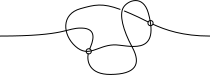
\includegraphics[width=0.40\textwidth, valign=c]{graphics/knot_welded_singular_example.pdf}
		\quad \overset{\sigma}{\longmapsto} \quad
		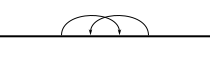
\includegraphics[width=0.40\textwidth, valign=c]{graphics/knot_welded_singular_example_arrow_diagram.pdf}
	\]
\end{example}

Just as in the classical case, there are natural relations to consider on arrow diagrams.

\begin{definition}
	A \textbf{long arrow Jacobi diagram} is an oriented unitrivalent graph where every trivalent vertex has at least one vertex oriented inward, and at least one oriented outwards, with the following additional data:
	\begin{itemize}
		\item at each trivalent vertex, a cyclic order of the incident edges,
		\item a fixed linear order on the univalent vertices.
	\end{itemize}
	modulo:
	\begin{enumerate}
		\item Six \textbf{directed STU} relations. For example,
		\begin{equation}
			\tag{\stu}
			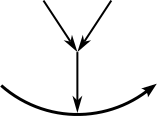
\includegraphics[width=0.10\textwidth, valign=c]{graphics/stu_welded_head_head_s.pdf}
			\quad
			=
			\quad
			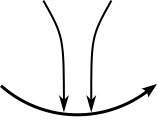
\includegraphics[width=0.10\textwidth, valign=c]{graphics/stu_welded_head_head_t.pdf}
			\quad
			-
			\quad
			\includegraphics[width=0.10\textwidth, valign=c]{graphics/stu_welded_head_head_u.pdf}.
		\end{equation}
		Relations hold for both choices of vertex type (two-heads-one-tail, one-head-two-tails) and all three choices of orientation of the trivalent vertex. Note that even though the skeleton is the line rather than the circle, we still draw it curved to distinguish it.
		\item Any \textbf{directed AS} relation. For example,
		\begin{equation}
			\tag{\as}
			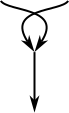
\includegraphics[width=0.05\textwidth, valign=c]{graphics/as_welded_head_head_a.pdf}
			\quad
			=
			\quad
			-
			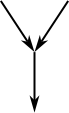
\includegraphics[width=0.05\textwidth, valign=c]{graphics/as_welded_head_head_s.pdf}.
		\end{equation}
		Again, for any choice of vertex type and rotation.
		\item Any \textbf{directed IHX} relations
		\begin{equation}
			\tag{\ihx}
			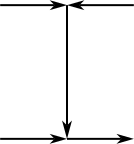
\includegraphics[width=0.10\textwidth, valign=c]{graphics/ihx_welded_example_i.pdf}
			\quad
			=
			\quad
			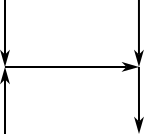
\includegraphics[width=0.10\textwidth, valign=c]{graphics/ihx_welded_example_h.pdf}
			\quad
			-
			\quad
			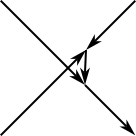
\includegraphics[width=0.10\textwidth, valign=c]{graphics/ihx_welded_example_x.pdf}.
		\end{equation}
		These hold for any compatible choice of both vertices in the diagrams.
		\item The \textbf{TC relation} (tails commute relation)
		\begin{equation}
			\label{eq:TC}
			\tag{\tc}
			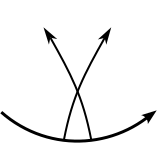
\includegraphics[width=0.10\textwidth, valign=c]{graphics/tc_relation_c.pdf}
			\quad
			=
			\quad
			-
			\includegraphics[width=0.10\textwidth, valign=c]{graphics/tc_relation_t.pdf}.
		\end{equation}
	\end{enumerate}
\end{definition}

The main difference between \(\mathcal{J}_{w}(|)\) and \(\mathcal{J}(|)\) is the tails commute relation which drastically reduces the complexity of the algebra.

\begin{proposition}[Two-in-one-out rule]
	In \(\mathcal{J}_{w}(|)\), any diagram containing a trivalent vertex with one vertex oriented inwards and two vertices oriented outward vanishes.
\end{proposition}

\begin{proof}
	Take such a diagram with a one-in-two-out vertex. Apply \ref{eq:STU}'s to all other vertices of the arrow diagram. The result is a sum of arrow diagrams, each containing a trivalent one-in-two-out vertex. We show that each such arrow diagram vasnishes. Since there is only one trivalent vertex in each diagram, the one-in-two-out vertex's incoming edge has its tail on the skeleton. Therefore applying the relevant \ref{eq:STU} relation equates the diagram with a difference of two diagrams that differ only by the order of placement of two tails on the skeleton. By \ref{eq:TC}, the difference is zero.
\end{proof}

Resultingly, only two versions of \ref{eq:STU}, one of \ref{eq:AS} and one of \ref{eq:IHX} remain nontrivial relations in \(\mathcal{J}_{w}(|)\).

\begin{warning}
	From this point it is clear when talking about welded objects we mean long welded objects. So, we write \(\mathcal{A}_{w}(|)\) as \(\mathcal{A}_{w}\), and don't necessarily specify that they are long.
\end{warning}

The existence of a finite type invariant \(Z\) for welded knots establishes a welded version of the fundamental theorem.

\begin{theorem}[\cite{finite-type-invariants-of-w-knotted-objects-I-w-knots-and-the-alexander-polynomial}]
	There exists a universal Vassiliev invariant \(Z_{w} : \mathcal{K}_{w} \to \mathcal{A}_{w}\).
\end{theorem}

Unlike the incredible involved construction for \(Z\), the construction of \(Z_{w}\) is relatively simple. The \ref{eq:TC} relation does all of the heavy lifting. A proof can be found in \cite{finite-type-invariants-of-w-knotted-objects-I-w-knots-and-the-alexander-polynomial}.

\begin{corollary}[Fundamental theorem of Vassiliev invariants of welded knots]
	We have
	\[\mathcal{A}_{w} \cong \gr \mathcal{A}_{w}.\]
	Equivalently,
	\[\mathcal{V}_{w} \cong \gr \mathcal{W}_{w}.\]
\end{corollary}
\section{Weight systems and Lie algebras}

There is a variant of Construction \ref{cons:lie-algebra-weight-system} for welded knots taking a Lie algebra and constructing a weight system. The difference is that vertices in string diagrams now have incoming edges (``heads'') and outgoing edges (``tails''), and diagramatically, only edges of the opposite orientation can be contracted. This was not true in the classical case, and the need to fix this is what made us restrict to metric Lie algebras. Hence, in the welded case we can consider any finite-dimensional Lie algebra.

Note an imporant difference to the classical case. There are now two types of univalent vertices that can connect to the external line: heads and tails. Heads correspond to elements of \(\mathfrak{g}\) and tails to elements of \(\mathfrak{g}^{\ast}\). Therefore, the role of \(\mathcal{U}(\mathfrak{g})\) in the classical case must be played here by some other associative algebra whose basis elements are words in \(\mathfrak{g} \sqcup \mathfrak{g}^{\ast}\).

Analysing the relations involving the external line should tell us what kind of object replaces \(\mathcal{U}(\mathfrak{g})\). From the two-in-one-out rule, there are three non-trivial cases to examine:
\[
	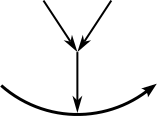
\includegraphics[width=0.10\textwidth, valign=c]{graphics/stu_welded_head_head_s.pdf} \; , \quad
	\includegraphics[width=0.10\textwidth, valign=c]{graphics/stu_welded_head_tail_s.pdf} \quad \text{and} \quad
	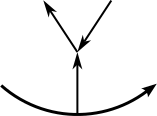
\includegraphics[width=0.10\textwidth, valign=c]{graphics/stu_welded_tail_head_s.pdf} \; .
\]
In all three cases, they obey commutator-like relations (the versions of \ref{eq:STU}), so the correct associative algebra target for the weight system is still the universal enveloping algebra of some Lie algebra. However since the connections to the external line can now be either heads or tails, representing elements of \(\mathfrak{g}\) and \(\mathfrak{g}^{\ast}\), the Lie algebra as a vector space is \(\mathfrak{g}^{\ast} \oplus \mathfrak{g}\).

Interpreting tails and heads in these \ref{eq:STU} relations as elements of \(\mathfrak{g}^{\ast} \oplus 0\) or \(0 \oplus \mathfrak{g}\) rather than \(\mathfrak{g}^{\ast}\) or \(\mathfrak{g}\) determines the bracket on \(\mathfrak{g}^{\ast} \oplus \mathfrak{g}\). For example, the \ref{eq:STU} with two heads on the external line implies that the bracket on \(0 \oplus \mathfrak{g}\) should be inherited from the bracket on \(\mathfrak{g}\).
\[
	\def\svgscale{0.3} \raisebox{-20pt}{\input{graphics/stu_welded_labelled_head_head_s.pdf_tex}}
	\quad
	=
	\quad
	\def\svgscale{0.3} \raisebox{-20pt}{\input{graphics/stu_welded_labelled_head_head_t.pdf_tex}}
	\quad
	-
	\quad
	\def\svgscale{0.3} \raisebox{-20pt}{\input{graphics/stu_welded_labelled_head_head_u.pdf_tex}}
\]
So, \([0 \oplus x, 0 \oplus y] = 0 \oplus [x, y]_{\mathfrak{g}}\).

To determine the bracket on \(\mathfrak{g}^{\ast} \oplus 0\), we need to examine one of the trivial cases not shown above. Indeed, the two-in-one-out rule neccecitates that the bracket on \(\mathfrak{g}^{\ast} \oplus 0\) be the zero-bracket. (Recall this rule was a consequence of the \ref{eq:TC} relation, and that \ref{eq:TC} stands for tails commute.)
\[
	\def\svgscale{0.3} \raisebox{-20pt}{\input{graphics/stu_welded_labelled_tail_tail_s.pdf_tex}}
	\quad
	=
	\quad
	\def\svgscale{0.3} \raisebox{-20pt}{\input{graphics/stu_welded_labelled_tail_tail_t.pdf_tex}}
	\quad
	-
	\quad
	\def\svgscale{0.3} \raisebox{-20pt}{\input{graphics/stu_welded_labelled_tail_tail_u.pdf_tex}}
	\quad
	=
	\quad
	0
\]
This gives \([\phi \oplus 0, \psi \oplus 0] = 0 \oplus 0\).

The bracket structure is known on the \(0 \oplus \mathfrak{g}\) and \(\mathfrak{g}^{\ast} \oplus 0\) direct summands, so the total Lie algebra structure will be a semidirect product \(\mathfrak{g}^{\ast} \rtimes \mathfrak{g}\), and what remains is to specify an action of \(\mathfrak{g}\) on \(\mathfrak{g}^{\ast}\). With a bit of work, the remaining `mixed' \ref{eq:STU} relations determine this. One such relation is
\[
	\def\svgscale{0.3} \raisebox{-20pt}{\input{graphics/stu_welded_labelled_head_tail_s.pdf_tex}}
	\quad
	=
	\quad
	\def\svgscale{0.3} \raisebox{-20pt}{\input{graphics/stu_welded_labelled_head_tail_t.pdf_tex}}
	\quad
	-
	\quad
	\def\svgscale{0.3} \raisebox{-20pt}{\input{graphics/stu_welded_labelled_head_tail_u.pdf_tex}}.
\]
Let us determine the functional \(\xi\) in terms of \(x\) and \(\psi\). There is only one type of nonzero trivalent vertex in \(\mathcal{A}_{w}\), so this is the same tensor as \(0 \oplus \mathfrak{g}\) case, just viewed from a different component. That tensor is \([\cdot, \cdot] \in \mathfrak{g}^{\ast} \otimes \mathfrak{g}^{\ast} \otimes \mathfrak{g}\) so \(\xi\) satisfies the equation \([\cdot, \cdot] = x^{\ast} \otimes \xi \otimes \phi^{\ast}\) whereby
\[[x, \xi^{\ast}] = \phi^{\ast} \quad \text{ so } \quad \phi([x, \xi^{\ast}]) = 1.\]
Therefore, \(\xi \in \mathfrak{g}^{\ast}\) is the functional
\[\xi : t \longmapsto \phi([x, t]).\]
This is also known as the \textbf{coadjoint action}, \(\xi = \operatorname{ad}^{\ast}_{x}(\phi)\) because it is the functional adjoint to \(\operatorname{ad}_{x}(\phi)\). Writing this in terms of the bracket on \(\mathfrak{g}^{\ast} \otimes \mathfrak{g}\),
\[[0 \oplus x, \psi \oplus 0] = \operatorname{ad}^{\ast}_{x}(\psi) \oplus 0.\]
Similarly, the \ref{eq:AS} relation gives \([\phi \oplus 0, 0 \oplus y] = -\operatorname{ad}^{\ast}_{y}(\phi) \oplus 0\). Hence, the total Lie algebra structure on \(\mathfrak{g}^{\ast} \oplus \mathfrak{g}\) is given by \(I\mathfrak{g}\) in the following definition.

\begin{definition}
	Let \(\mathfrak{g}\) be a finite-dimensional Lie algebra, and let \(\mathfrak{g}^{\ast}\) denote the vector space \(\mathfrak{g}^{\ast}\) with the structure of an abelian Lie algebra. Then let \(I\mathfrak{g}\) denote the Lie algebra \(\mathfrak{g}^{\ast} \rtimes \mathfrak{g}\) with the bracket
	\[[\phi \oplus x, \psi \oplus y] = \operatorname{ad}^{\ast}_{x}(\psi) - \operatorname{ad}^{\ast}_{y}(\phi) \oplus [x, y].\]
\end{definition}
\begin{remark}
	This construction coincides with the Drinfeld double \cite{quantum-groups} of the Lie bialgebra \(\mathfrak{g}\), in the case where \(\mathfrak{g}\) is co-commutative.
\end{remark}

\begin{proposition}
	There is a well-defined algebra homomorphism \(\mathcal{A}_{w} \to \mathcal{U}(I\mathfrak{g})\) given by a variant of Construction \ref{cons:lie-algebra-weight-system}.
\end{proposition}

\begin{proof}
	The relations in \(\mathcal{A}_{w}\) are generated by \ref{eq:STU} and \ref{eq:TC}. We have shown that these relations are also true in \(\mathcal{U}(I\mathfrak{g})\).
\end{proof}

\section{The universal welded weight system}

The aim of this section is to prove a Hinnich-Vaintrob style statement for \(\mathcal{A}_{w}\).

\begin{definitions}
	An \(n\)-\textbf{coloured prop} is a symmetric monoidal category generated by \(n\) objects.
\end{definitions}

The definition of an algebra over a prop (Definition \ref{def:algebra-over-prop}) extends naturally to coloured props as well.

\begin{definition}
	\label{def:2-coloured-casimir-prop}
	We define a two-coloured prop \(\mathbf{T}_{m}\). Its generating objects are \(\mathbf{1}\) and \(\mathbf{1}^{\vee}\). Denote the objects \(\mathbf{1}^{\otimes n}\) and \((\mathbf{1}^{\vee})^{\otimes n}\) as \(\mathbf{n}\) and \(\mathbf{n}^{\vee}\) respectively, as well as \((\mathbf{1}^{\vee})^{\otimes n} \otimes \mathbf{1}^{\otimes k}\) as \(\mathbf{n}^{\vee} + \mathbf{k}\).

	The symmetric monoidal category \(\mathbf{T}_{m}\) generating morphisms
	\[
		\mathbf{T}_{m}(\mathbf{k}, \mathbf{n})
		=
		\bigoplus_{f: [k] \to [n]}
		\bigotimes_{i = 1}^{n}
		\mathcal{O}_{\text{Lie}}(|f^{-1}(i)|)
		,
	\]
	as well as \(c \in \mathbf{T}_{m}(\mathbf{0}, \mathbf{1}^{\vee} + \mathbf{1})\) and \(m \in \mathbf{T}_{m}(\mathbf{1}^{\vee} + \mathbf{1}, \mathbf{0})\)
	satisfying the relations induced by \(\mathcal{O}_{\text{Lie}}\) and the relations
	\[(\id_{\mathbf{1}} \otimes c) \circ (m \otimes \id_{\mathbf{1}}) = \id_{\mathbf{1}}\]
	and
	\[(c \otimes \id_{\mathbf{1}^{\vee}}) \circ (\id_{\mathbf{1}^{\vee}} \otimes m) = \id_{\mathbf{1}^{\vee}}\]
	(that is, \(\mathbf{1}\) and \(\mathbf{1}^{\vee}\) are rigid with coevaluation and evaluation maps \(c\) and \(m\) respectively).
\end{definition}

In view of the difference between \(\mathcal{U}(\mathfrak{g})\) and \(\mathcal{U}(I\mathfrak{g})\), the category \(\mathbf{T}_{m}\) generalises the metric envelope of the Lie operad \(\mathbf{E}_{m}(\mathcal{O}_{\text{Lie}})\) to include as objects both tensor powers of \(\mathfrak{g}\) but also tensor powers of \(\mathfrak{g}^{\ast}\). In terms of string diagrams, the string diagrams that describe \(\mathbf{T}_{m}\) are oriented, so they have heads and tails. The property of \(\mathbf{E}_{m}(\mathcal{O}_{\text{Lie}})\) to describe the internal structure of \(\mathcal{A}\) is thus generalised to \(\mathcal{A}_{w}\), whose internal structure is described by \(\mathbf{T}_{m}\).

Again however, there is the problem that \(\mathbf{T}_{m}\) also describes arrow diagrams with no univalent vertices. Recall that the motivation behind Definition \ref{def:casimir-envelope-of-cyclic-operad} was to exclude the metric morphism as not to describe chord diagrams with no univalent vertices. The motivation for the following definition is similar.

\begin{definition}
	The symmetric monoidal category \(\mathbf{T}_{c}\) is the symmetric monoidal subcategory of \(\mathbf{T}_{m}\) generated by the morphisms \(\beta\) and \(c\) (but not \(m\)) as well as the morphisms
	\[
		a_{\ell}
		=
		(\id_{\mathbf{1}^{\vee}} \otimes m)
		\circ
		(\id_{\mathbf{1}^{\vee}} \otimes \beta \otimes \id_{\mathbf{1}^{\vee}})
		\circ
		(c \otimes \id_{\mathbf{1}} \otimes \id_{\mathbf{1}^{\vee}})
	\]
	and
	\[
		a_{r}
		=
		((m \circ \tau) \otimes \id_{\mathbf{1}^{\vee}})
		\circ
		(\id_{\mathbf{1}^{\vee}} \otimes \beta \otimes \id_{\mathbf{1}^{\vee}})
		\circ
		(\id_{\mathbf{1}^{\vee}} \otimes \id_{\mathbf{1}} \otimes (c \circ \tau))
	\]
	which in terms of string diagrams are
	\[
		{\scriptsize
		\def\svgscale{0.38}
		\adjustbox{valign=c}{\input{graphics/two_coloured_coadjoint_action_left.pdf_tex}}
		}
		\qquad
		\text{and}
		\qquad
		{\scriptsize
		\def\svgscale{0.38}
		\adjustbox{valign=c}{\input{graphics/two_coloured_coadjoint_action_right.pdf_tex}}
		}
	\]
	respectively.
\end{definition}

Denote \(\mathbf{I} = \mathbf{1}^{\vee} \oplus \mathbf{1} \in \mathbf{T}_{c}\). We will define a morphism \(y: \mathbf{I} \otimes \mathbf{I} \to \mathbf{I}\) that makes \(\mathbf{I}\) into a Lie algebra object in \(\mathbf{T}_{c}\). Note that by the \(k\)-linearity of \(\mathbf{T}_{c}\), a map of sigature \(\mathbf{I} \otimes \mathbf{I} \to \mathbf{I}\) is determined by eight maps of similar signature between objects \(\mathbf{1}^{\vee}\) or \(\mathbf{1}\). Indeed expanding \(\mathbf{I} = \mathbf{1}^{\vee} \oplus \mathbf{1}\), we get that
\[
	y
	:
	(\mathbf{1}^{\vee} \otimes \mathbf{1}^{\vee})
	\oplus
	(\mathbf{1}^{\vee} \otimes \mathbf{1})
	\oplus
	(\mathbf{1} \otimes \mathbf{1}^{\vee})
	\oplus
	(\mathbf{1} \otimes \mathbf{1})
	\longrightarrow
	\mathbf{1}^{\vee} \oplus \mathbf{1}
	.
\]

\begin{proposition}
	Let \(y: \mathbf{I} \otimes \mathbf{I} \to \mathbf{I}\) be the morphism whose only nonzero components in the above decomposition are in components \({\mathbf{1} \otimes \mathbf{1} \to \mathbf{1}}\), \({\mathbf{1} \otimes \mathbf{1}^{\vee} \to \mathbf{1}^{\vee}}\) and \({\mathbf{1}^{\vee} \otimes \mathbf{1} \to \mathbf{1}^{\vee}}\) and let it be given by
	\[
		y = \beta \oplus a_{\ell} \oplus a_{r}.
	\]
	Then \(\mathbf{I}\) is a Lie algebra object of \(\mathbf{T}_{c}\) with morphism \(y\).
\end{proposition}

\begin{proof}
	We have
	\[
		y
		\quad
		=
		\quad
		{\scriptsize
		\def\svgscale{0.38}
		\adjustbox{valign=c}{\input{graphics/two_coloured_bracket.pdf_tex}}
		}
		\quad
		+
		\quad
		{\scriptsize
		\def\svgscale{0.38}
		\adjustbox{valign=c}{\input{graphics/two_coloured_coadjoint_action_left.pdf_tex}}
		}
		\quad
		+
		\quad
		{\scriptsize
		\def\svgscale{0.38}
		\adjustbox{valign=c}{\input{graphics/two_coloured_coadjoint_action_right.pdf_tex}}
		}
		\quad
	\]
	(where here the trivalent vertex is \(\beta\)). There are two statements to prove:
	\begin{enumerate}
		\item
			\label{prf:generalised-antisymmetry-y}
			The generalised antisymmetry of \((\mathbf{I}, y)\), namely
			\[y + y \circ \tau = 0\]
		\item
			\label{prf:generalised-jacobi-y}
			The generalised Jacobi identity of \((\mathbf{I}, y)\), namely
			\[(y \circ (y \otimes \id_{\mathbf{I}})) \circ (1 + \tau_{123} + \tau_{132}) = 0.\]
	\end{enumerate}

	For the proof of \ref{prf:generalised-antisymmetry-y}, observe that \(t + y \circ \tau\) contains six terms:
	\(\beta + \beta \circ \tau \in \mathbf{T}_{c}(\mathbf{1} \otimes \mathbf{1}, \mathbf{1})\),
	\(a_{\ell} + a_{r} \circ \tau \in \mathbf{T}_{c}(\mathbf{1} \otimes \mathbf{1}^{\vee}, \mathbf{1}^{\vee})\) and
	\(a_{r} + a_{\ell} \circ \tau \in \mathbf{T}_{c}(\mathbf{1}^{\vee} \otimes \mathbf{1}, \mathbf{1})\).
	It suffices to check that each of these components are zero.

	In the component \(\mathbf{T}_{c}(\mathbf{1} \otimes \mathbf{1}, \mathbf{1})\), we have \(\beta + \beta \circ \tau = 0\). This relation is simply the antisymmetry of the bracket \(\beta\) (with which \(\mathbf{1}\) is a Lie algebra object in \(\mathbf{T}_{c}\)) --- in terms of string diagrams this is
	\[
		\quad
		{\scriptsize
		\def\svgscale{0.38}
		\adjustbox{valign=c}{\input{graphics/two_coloured_bracket.pdf_tex}}
		}
		\quad
		+
		\quad
		{\scriptsize
		\def\svgscale{0.38}
		\adjustbox{valign=c}{\input{graphics/two_coloured_bracket_braided.pdf_tex}}
		}
		\quad
		=
		\quad
		0
		.
	\]

	We also have \(a_{\ell} + a_{r} \circ \tau \in \mathbf{T}_{c}(\mathbf{1} \otimes \mathbf{1}^{\vee}, \mathbf{1}^{\vee})\). Diagramatically this is
	\[
		\quad
		{\scriptsize
		\def\svgscale{0.38}
		\adjustbox{valign=c}{\input{graphics/two_coloured_coadjoint_action_left.pdf_tex}}
		}
		\quad
		+
		\quad
		{\scriptsize
		\def\svgscale{0.38}
		\adjustbox{valign=c}{\input{graphics/two_coloured_coadjoint_action_right_braided.pdf_tex}}
		}
		\quad
		\in \mathbf{T}_{c}(\mathbf{1} \otimes \mathbf{1}^{\vee}, \mathbf{1}^{\vee})
		.
	\]
	Substituting
	\[
		\quad
		{\scriptsize
		\def\svgscale{0.38}
		\adjustbox{valign=c}{\input{graphics/two_coloured_bracket.pdf_tex}}
		}
		\quad
		=
		\quad
		-
		\quad
		{\scriptsize
		\def\svgscale{0.38}
		\adjustbox{valign=c}{\input{graphics/two_coloured_bracket_braided.pdf_tex}}
		}
	\]
	into the first term, we get
	\[
		-
		\quad
		{\scriptsize
		\def\svgscale{0.38}
		\adjustbox{valign=c}{\input{graphics/two_coloured_coadjoint_action_left_with_twist_inserted.pdf_tex}}
		}
		\quad
		=
		\quad
		{\scriptsize
		\def\svgscale{0.38}
		\adjustbox{valign=c}{\input{graphics/two_coloured_coadjoint_action_right_braided.pdf_tex}}
		}
		\quad
		\in \mathbf{T}_{c}(\mathbf{1} \otimes \mathbf{1}^{\vee}, \mathbf{1}^{\vee})
		.
	\]
	Indeed, the two diagrams are equal and therefore their difference is zero. This follows from the relation
	\[
		\quad
		{\scriptsize
		\def\svgscale{0.38}
		\adjustbox{valign=c}{\input{graphics/two_coloured_bracket_equivariance.pdf_tex}}
		}
		\quad
		=
		\quad
		-
		\quad
		{\scriptsize
		\def\svgscale{0.38}
		\adjustbox{valign=c}{\input{graphics/two_coloured_bracket_equivariance_simplified.pdf_tex}}
		}
	\]
	which is a consequence of the fact that morphisms in \(\mathbf{T}_{c}\) are direct sums of elements of \(\mathcal{O}_{\text{Lie}}\) (Definition \ref{def:2-coloured-casimir-prop}), and the equivariance axioms of the Lie operad in Definition \ref{def:operad}.

	Without loss of generality, the same argument proves that \(a_{r} + a_{\ell} \circ \tau = 0 \in \mathbf{T}_{c}(\mathbf{1}^{\vee} \otimes \mathbf{1}, \mathbf{1})\), completing the proof of \ref{prf:generalised-antisymmetry-y}.

	Continuing on to the proof of \ref{prf:generalised-jacobi-y}, we first compute \(y \circ (y \otimes \id_{\mathbf{I}})\). There are nine terms to consider, but some vanish due to being in different components of the direct sum --- only those terms where the output object of the first morphism matches the input morphism of the second morphism are non-zero. Take for example \(a_{r} \circ (\beta \otimes \id_{\mathbf{I}}) = 0\). Of the nine terms, only four fail to vanish for this reason. Namely,
	\[
		y \circ (y \otimes \id_{\mathbf{I}})
		=
		\beta \circ (\beta \otimes \id_{\mathbf{I}})
		+
		\beta \circ (a_{\ell} \otimes \id_{\mathbf{I}})
		+
		a_{\ell} \circ (a_{r} \otimes \id_{\mathbf{I}})
		+
		a_{r} \circ (a_{r} \otimes \id_{\mathbf{I}})
		.
	\]
	The string-diagrammatic version of this expression is
	\[
		\mspace{9mu}
		{\tiny
		\def\svgscale{0.30}
		\adjustbox{valign=c}{\input{graphics/two_coloured_double_bracket_term_1.pdf_tex}}
		}
		\mspace{9mu}
		+
		\mspace{9mu}
		{\tiny
		\def\svgscale{0.30}
		\adjustbox{valign=c}{\input{graphics/two_coloured_double_bracket_term_2.pdf_tex}}
		}
		\mspace{9mu}
		+
		\mspace{9mu}
		{\tiny
		\def\svgscale{0.30}
		\adjustbox{valign=c}{\input{graphics/two_coloured_double_bracket_term_3.pdf_tex}}
		}
		\mspace{9mu}
		+
		\mspace{9mu}
		{\tiny
		\def\svgscale{0.30}
		\adjustbox{valign=c}{\input{graphics/two_coloured_double_bracket_term_4.pdf_tex}}
		}
		\mspace{9mu}
		.
	\]
	It remains to show precomposing this expression with \((1 + \tau_{123} + \tau_{132})\) gives the zero morphism from \(\mathbf{I} \otimes \mathbf{I} \otimes \mathbf{I} \to \mathbf{I}\).

	Indeed, for the first term we have
	\[\beta \circ (\beta \otimes \id_{\mathbf{I}}) \circ (1 + \tau_{123} + \tau_{132})  = 0\]
	from the fact that \(\mathbf{1}\) is a Lie algebra object with morphism \(\beta\).

	Note here that if \(\mathbf{x}, \mathbf{y}, \mathbf{z} \in \{\mathbf{1}, \mathbf{1}^{\vee}\}\) and \(f: \mathbf{x} \otimes \mathbf{y} \otimes \mathbf{z} \to \mathbf{1}^{\vee}\) then \(f \circ (1 + \tau_{123} + \tau_{132})\) has components in \(\mathbf{x} \otimes \mathbf{y} \otimes \mathbf{z} \to \mathbf{1}^{\vee}\), \(\mathbf{y} \otimes \mathbf{z} \otimes \mathbf{x} \to \mathbf{1}^{\vee}\) and \(\mathbf{z} \otimes \mathbf{x} \otimes \mathbf{y} \to \mathbf{1}^{\vee}\). Therefore, the analysis with the remaining three terms is not as simple, as the domains are not cyclically invariant tensor products in \(\{\mathbf{1}, \mathbf{1}^{\vee}\}\).

	It remains to show that
	\[(\beta \circ (a_{\ell} \otimes \id_{\mathbf{I}}) + a_{\ell} \circ (a_{r} \otimes \id_{\mathbf{I}}) + a_{r} \circ (a_{r} \otimes \id_{\mathbf{I}})) \circ (1 + \tau_{123} + \tau_{132})\]
	vanishes. This morphism in \(\mathbf{T}_{c}(\mathbf{I} \otimes \mathbf{I} \otimes \mathbf{I}, \mathbf{I})\) only has components in \(\mathbf{T}_{c}(\mathbf{1} \otimes \mathbf{1} \otimes \mathbf{1}^{\vee}, \mathbf{1}^{\vee})\), \(\mathbf{T}_{c}(\mathbf{1} \otimes \mathbf{1}^{\vee} \otimes \mathbf{1}, \mathbf{1}^{\vee})\) and \(\mathbf{T}_{c}(\mathbf{1}^{\vee} \otimes \mathbf{1} \otimes \mathbf{1}, \mathbf{1}^{\vee})\) so it suffices to check these components.

	We provide the calculation in the \(\mathbf{T}_{c}(\mathbf{1} \otimes \mathbf{1} \otimes \mathbf{1}^{\vee}, \mathbf{1}^{\vee})\) component --- the proof that the other components follow from similar arguments. Indeed in \(\mathbf{T}_{c}(\mathbf{1} \otimes \mathbf{1} \otimes \mathbf{1}^{\vee}, \mathbf{1}^{\vee})\) we have the contributions
	\[
		\beta \circ (a_{\ell} \otimes \id_{\mathbf{I}}) \circ 1
		+
		a_{\ell} \circ (a_{r} \otimes \id_{\mathbf{I}}) \circ \tau_{132}
		+
		a_{r} \circ (a_{r} \otimes \id_{\mathbf{I}}) \circ \tau_{123}
		.
	\]
	Diagramatically, that is
	\[
		\mspace{9mu}
		{\tiny
		\def\svgscale{0.30}
		\adjustbox{valign=c}{\input{graphics/two_coloured_double_bracket_component_11v_term_2_id.pdf_tex}}
		}
		\mspace{9mu}
		+
		\mspace{9mu}
		{\tiny
		\def\svgscale{0.30}
		\adjustbox{valign=c}{\input{graphics/two_coloured_double_bracket_component_11v_term_3_perm132.pdf_tex}}
		}
		\mspace{9mu}
		+
		\mspace{9mu}
		{\tiny
		\def\svgscale{0.30}
		\adjustbox{valign=c}{\input{graphics/two_coloured_double_bracket_component_11v_term_4_perm123.pdf_tex}}
		}
		\mspace{9mu}
		.
	\]
	Simplifying these terms via the rigidity relations of Definiton \ref{def:internal-to-additive-monoidal-category} \ref{def:rigid-category-and-object} as well as the antisymmetry of the bracket \(\beta\), we arrive at
	\[
		\mspace{9mu}
		{\tiny
		\def\svgscale{0.30}
		\adjustbox{valign=c}{\input{graphics/two_coloured_double_bracket_component_11v_term_2_id_simplified.pdf_tex}}
		}
		\mspace{9mu}
		+
		\mspace{9mu}
		{\tiny
		\def\svgscale{0.30}
		\adjustbox{valign=c}{\input{graphics/two_coloured_double_bracket_component_11v_term_3_perm132_simplified.pdf_tex}}
		}
		\mspace{9mu}
		+
		\mspace{9mu}
		{\tiny
		\def\svgscale{0.30}
		\adjustbox{valign=c}{\input{graphics/two_coloured_double_bracket_component_11v_term_4_perm123_simplified.pdf_tex}}
		}
		\mspace{9mu}
	\]
	(specifically, the first and third terms are simplified only by the rigidity relations, while the second term is simplified by the rigidity relations and two applications of the antisymmetry of \(\beta\)). Finally, \(\beta\) is a Lie algebra object in \(\mathbf{T}_{c}\), and since the three terms in this expression factor through the generalised Jacobi identity for \(\beta\), we have
	\[
		\mspace{9mu}
		{\tiny
		\def\svgscale{0.30}
		\adjustbox{valign=c}{\input{graphics/two_coloured_double_bracket_component_11v_term_2_id_simplified.pdf_tex}}
		}
		\mspace{9mu}
		+
		\mspace{9mu}
		{\tiny
		\def\svgscale{0.30}
		\adjustbox{valign=c}{\input{graphics/two_coloured_double_bracket_component_11v_term_3_perm132_simplified.pdf_tex}}
		}
		\mspace{9mu}
		+
		\mspace{9mu}
		{\tiny
		\def\svgscale{0.30}
		\adjustbox{valign=c}{\input{graphics/two_coloured_double_bracket_component_11v_term_4_perm123_simplified.pdf_tex}}
		}
		\mspace{9mu}
		=
		\mspace{9mu}
		0
	\]
	completing the proof.
\end{proof}

\begin{corollary}
	\label{cor:universal-two-coloured-casimir-envelope-arrow-diagrams-isomorphism}
	Let \(\mathbf{I}\) denote the Lie algebra object \(\mathbf{1} \oplus \mathbf{1}^{\vee}\) (with the morphism \(y\)) in the two-coloured prop \(\mathbf{T}_{c}\). The bialgerba \(U(\mathcal{O}_{\text{Lie}}, \mathbf{I})\) is isomorphic to \(\mathcal{A}_{w}\) as a filtered bialgebra.
\end{corollary}

\begin{proof}
	The proof proceeds verbatim to the proof of Theorem \ref{thm:universal-casimir-lie-envelope-chord-diagrams-isomorphism}, but with \(\mathcal{A}\) replaced by \(\mathcal{A}_{w}\) and with \(\mathbf{1}\) replaced by \(\mathbf{I}\).
\end{proof}

A philosophical interepretation of this theorem is that the algebra \(\mathcal{A}_{w}\) behaves like the universal enveloping algebra \(\mathcal{U}(I\mathfrak{g})\) of a cocommutative Drinfeld double \(I\mathfrak{g}\).

Furthermore, for classical weight systems Theorem \ref{thm:universal-casimir-lie-envelope-chord-diagrams-isomorphism} proves that every weight system (so every functional on \(\mathcal{A}\)) comes from applying Construction \ref{cons:lie-algebra-weight-system} to some Lie algebra object in some symmetric monoidal category. For welded weight systems, this already follows from \cite[Theorem 3.26]{finite-type-invariants-of-w-knotted-objects-I-w-knots-and-the-alexander-polynomial} which states that the universal finite type invariant of welded knots contains exactly the same information as the Alexander polynomial, and recall that the Alexander polynomial factors through the weight system \(W_{\mathfrak{gl}_{1|1}}\). Since every welded weight system factors through \(Z_{w}\), they all constructible via Construction \ref{cons:lie-algebra-weight-system} applied to the Lie superalgebra \(\mathfrak{gl}_{1|1}\). Corollary \ref{cor:universal-two-coloured-casimir-envelope-arrow-diagrams-isomorphism} gives an alternative, categorical proof of this fact.

\begin{shaded}
	Actually \cite[Theorem 3.26]{finite-type-invariants-of-w-knotted-objects-I-w-knots-and-the-alexander-polynomial} says that the \(Z\) for welded knots is Alexander polynomial plus self-linking numbers (so I guess, Milnor invariants?) (arrow diagrams that are trees).

	The Alexander polynomial factors through \(\mathfrak{gl}_{1|1}\), but what about Milnor invariants. My intuition tells me that trees should come from Lie algebras in which case the triviality still holds. Zsuzsi --- do you know if this is true?
\end{shaded}
